\documentclass{sp}

% The \pdf* commands provide metadata for the PDF output.
% Do not use LaTeX style / commands like \emph{} inside these.
\pdfauthor{Author Full Name(s)}
\pdftitle{The role of priors, competence and relevance for the interpretation of disjunction}
\pdfkeywords{exclusive disjunction, scalar implicature, pragmatics}

%%%%%%%%%%%%%%%%%%%%%%%%%%%%%%%%%%%%%%%%%%%%%%%%%%
%% customization
%%%%%%%%%%%%%%%%%%%%%%%%%%%%%%%%%%%%%%%%%%%%%%%%%%
\usepackage{gb4e}
\noautomath
\usepackage[dvipsnames]{xcolor}
\usepackage{multirow,booktabs}
\newcommand{\mf}[1]{\textcolor{BurntOrange}{[MF: #1]}}
\newcommand{\pt}[1]{\textcolor{Cerulean}{[PT: #1]}}
\newcommand{\bvt}[1]{\textcolor{ForestGreen}{[BvT: #1]}}

% Optional short title inside square brackets, for the running headers.
% If no short title is given, no title appears in the headers.
\title[Exclusive disjunction]{The role of priors, competence and relevance for the interpretation of disjunction%
  \thanks{We thank \ldots}}

% Optional short author inside square brackets, for the running headers.
% If no short author is given, no authors print in the headers.
\author[]{% As many authors as you like, each separated by \AND.
  \spauthor{Polina Tsvilodub \\ \institute{Institute}} \AND
  \spauthor{Bob van Tiel \\ \institute{Institute}} \AND
  \spauthor{Michael Franke \\ \institute{Department of Linguistics \\ University of Tübingen}}}

\begin{document}

\maketitle

\begin{abstract}
  
  Sentences containing disjunctions like ``Donald ate a pretzel or a donut'' are often taken as conveying that Donald ate a pretzel or a donut, but not both. That is, the listener might infer an \textit{exclusive reading of the disjunction}. Current standard accounts of disjunction interpretation posit that the exclusive interpretation of disjunctions is an instance of \textit{scalar implicature}. Prior work suggests that, among others, three factors influence the robustness of scalar implicatures: (i) \textit{relevance} of the stronger alternative to the listener, (ii) the \textit{competence} of the speaker about the truth of the stronger alternative, and (iii) the \textit{prior probability} that the stronger alternative is true. While their influence was investigated experimentally for the interpretation of ``some'', the evidence is less conclusive in the case of disjunction interpretation. Therefore, we compare experimentally the interpretation of ``some'' and ``or'', while manipulating the three factors with respect to the stronger alternatives “all”, and “and”, respectively. Our results indicate that competence has a consistent effect of the robustness of the implicature generation for both triggers, while prior and relevance exhibit different, more intricate, effects varying between the triggers.
  
\end{abstract}

\begin{keywords}
 exclusive disjunction, scalar implicature, pragmatics
\end{keywords}

\section{Introduction}

\pt{Framing suggestion: start out with a general introduction on scalar implicature as applicable to both some and or,  give some details on why xor is also interesting. Ported over from abstract. Review prior work focusing on separate factors influencing SIs. Motivate our study.}

If someone says “Anna ate some cookies”, the hearer might infer the upper-bounded reading that Anna ate some, but not all cookies. Modern theories usually treat this inference as one of the prime examples of \textit{scalar implicature} (SI) \citep{horn1972semantic}. More specifically, the SI relies on a lexical scale consisting of words ordered in terms of informativeness (or, strength), like $\langle$some, all$\rangle$. When interlocutors encounter the weaker expression ``some'', the stronger ``all'' functions as a salient alternative \citep{matsumoto1995conversational}. 

Theories of pragmatics suggest that interlocutors reason about these scales, guided by conversational principles introduced by \citet{grice1975logic}.
According to \citet{grice1975logic}, natural conversation is governed by
the assumption that speakers are cooperative; that is, they attempt to further the purpose
of the discourse by means of their utterances. Speakers are cooperative by adhering
to four maxims that enjoin their utterances to be truthful, informative, relevant,
and clear. Sometimes hearers have to make ancillary assumptions in order to align a
speaker’s utterance with the assumption of cooperativity. Such ancillary assumptions
are called conversational implicatures.
%Recent theories of pragmatics suggest that cooperative interlocutors reason about each other's utterances, guided by certain \textit{conversational maximes} \citep{grice1975logic}. 
That is, in case of ``some'', assuming a rational speaker who wishes to be maximally cooperative, the listener of the utterance would infer that if the stronger alternative (i.e., ``all'') was true, the speaker would have used the stronger utterance; but since she did not, she must have lacked the evidence for using ``all''P.

Similarly to the first example, given the utterance “Donald ate a donut or a pretzel.”, the listener might infer that Donald ate either the donut or the pretzel, but not both (i.e., an \textit{exclusive} interpretation).
%This inference can also be explained as a variety of scalar implicature, relying on the scale $\langle$or, and$\rangle$. If a speaker uses an informationally weaker term (e.g., “some”), they may imply that the corresponding stronger alternative (e.g., “and”) is false [3,5]. 
\pt{ported over from old paper below}
 
Introductions to logic usually distinguish between two readings of “or”: an inclusive
and an exclusive reading (e.g., McCawley, 1981; Copi \& Cohen, 2005). The inclusive
reading corresponds to the meaning of logical disjunction. According to this reading,
“A or B” is true if at least one and possibly both of A and B are true. The exclusive
reading is more strict in that it excludes the possibility that both A and B are true. So
on its exclusive reading, “A or B” is true if exactly one of A and B is true. 

The standard account of exclusive readings of disjunction in the literature also stems from Grice’s (1975) theory of conversational implicature (e.g., Chevallier, Noveck, Nazir, Bott, Lanzetti, \& Sperber, 2008; Chierchia, Fox, \& Spector, 2012; Geurts, 2010; Sauerland, 2004). 
\citet{horn1972semantic} was the first to argue that the exclusive reading of “or” can be explained as a conversational implicature, too, based on the assumption that the primary meaning of “or” is inclusive. To illustrate, consider (1) again. Assuming that the primary
meaning of “or” is inclusive, the speaker of (1) could have been more informative,
and hence cooperative, by uttering the “and”-alternative “Joe supports Donald
and Hillary.” Why didn’t she? Presumably because she does not believe that the “and”-
alternative is true. This is a weak inference that is compatible with a situation in which
the speaker is unsure about whether or not Joe supports both Donald and Hillary. This
weak inference can be strengthened if there is reason to believe that the speaker knows
whether or not Joe supports both Donald and Hillary. This assumption is often called
the competence assumption (e.g., Geurts, 2010; Russell, 2006; Schulz \& van Rooij,
2006; Zimmermann, 2000). If the competence assumption is sufficiently plausible, it
follows that, according to the speaker, Joe does not support both Donald and Hillary.
For this conversational implicature it is assumed that “or” forms a lexical scale with “and” %, and that alternatives are generated by substituting the scalemates “or” and “and”. Other lexical scales are <some, all>, <warm, hot>, and <intelligent, brilliant>.

Alternative theories propose that the presence of these two readings might suggest that “or” is associated with two
different lexical entries (e.g., Basson \& O’Connor, 1960; Baum, 1996; Rescher, 1964).
There are, however, good reasons to reject such a lexicalist approach. Perhaps the most
compelling reason is that, in some contexts, “or” can only receive one interpretation.
To illustrate, consider the following sentence, in which “or” occurs in the scope of
negation: (2) Joe does not support Donald or Hillary.
This sentence has only one interpretation, namely that Joe supports neither Donald nor
Hillary (cf. Crain, 2008). This interpretation corresponds to the inclusive reading of
“or”. It does not have an interpretation corresponding to the exclusive reading; in other
words, it does not have a reading according to which Joe either supports both Donald
and Hillary, or neither of them. Since “or” is systematically monosemous in certain
contexts—negation being one of them—it follows that the two readings of “or” cannot
simply be due to a lexical ambiguity.

The implicature account straightforwardly explains the absence of exclusive readings
under negation. Consider (2) again. Here, unlike in the case of (1), the “and”-
alternative is less informative than the utterance itself. After all, (2) is only compatible
with a situation in which Joe supports neither Donald nor Hillary, whereas the
“and”-alternative is also consistent with situations in which Joe supports exactly one
of Donald and Hillary. So the speaker was already maximally informative and hence
no implicature is derived.
Although the implicature account has since become the standard in the literature
(e.g., Chevallier, Noveck, Nazir, Bott, Lanzetti, \& Sperber, 2008; Chierchia, Fox, \&
Spector, 2012; Geurts, 2010; Sauerland, 2004), it is not without its problems, as we
will see in the next section. 
\pt{end of section from old paper}

Crucially, prior research suggests that the robustness of SIs is influenced by different contextual factors.

\subsection{Scalar implicature}

\textbf{Related experimental/modelling work: } 
Some: \citep{degen2015investigating, goodman2016pragmatic}, 
Or: \citep{Li2021}

\section{Relevance, competence and prior pribability}
Literature on the effects of these factors on SIs \citep{sperber1986relevance, goodman2013knowledge, degen2015wonky}. 
\subsection{Relevance}

\subsection{Competence}

\subsection{Prior probability}

\subsection{Predictions}
Prior research has shown that the robustness of implicatures from ``some'' to ``some, but not all''  predicted by the standard scalar implicature (SI) account is influenced by three factors. First, high contextual relevance of the stronger alternative ``all'' to the listener is predicted to render more robust scalar implicatures. Second, high speaker competence about the truth of the stronger alternative is predicted to lead to more robust scalar implicature generation. Lastly, high prior probability of the stronger ``all'' being true is assumed to \textit{decrease} the scalar implicature rate. \pt{If the framing is okay, add some motivation and predictions regarding investigating the conjunction of these factors.} \mf{yes, good idea}
If the currently standard scalar implicature account also holds for the interpretation of disjunctions, analogous predictions for the robustness of the implicature from ``A or B'' to ``A or B, but not both'' can be derived. In case of disjunction, the relevant stronger alternative is ``and''.

We hypothesize that all three factors influence the robustness of scalar implicatures for both triggers. That is, we expect a higher rate of endorsements for sentences containing the upper-bounded (exclusive, in case of ``or'') paraphrases of the respective triggers when the three factors are intuitively judged to be high or low, as described above. We, therefore, test six hypotheses, one concerning the effect of each factor for each trigger. 
Simultaneously,  we also address the \textit{identity hypothesis} that exclusive readings of disjunctions are a scalar implicature just like the ``some → some but not all'' case. If the identity hypothesis is correct, we expect that whichever factors positively or negatively affect the implicature readings of ``some'', exactly these factors also affect the exclusive readings of ``or''. In other words, the prediction of the identity hypothesis could still be confirmed even if the hypotheses related to the effects of relevance, competence and prior are not borne out, as long as the observed results are the same for ``some'' and ``or''. To investigate this, we directly compare the interpretation of the two triggers within one experiment, described in the following section.

\section{Experiment}

In this experiment we directly compare the interpretation of ``some'' and ``or'', so as to explore if the predictions generated by the scalar implicature account are borne out comparably for both triggers. Specifically, we manipulate the \textit{contextual relevance of the stronger alternative to the listener}, the \textit{speaker's competence about the truth of ``all'' / ``and''}, and the \textit{prior probability of ``all'' / ``and'' being true}, to investigate the robustness of an exclusive reading of ``or'' (``A or B, but not both'') under these manipulations, in direct comparison to the upper-bounded reading of “some” (``some but not all'').

\mf{The exposition of the experiment meanders quite a bit between high-level description, materials and procedure. I would advocate a tidier organization: high-level, materials, then procedure.}

To operationalize these factors, we designed context stories (vignettes) which were judged to score either high or low with respect to each factor of interest (high/low prior probability of the more informative alternative $\times$ high/low speaker competence $\times$ high/low contextual relevance of the alternative). Combining these dichotomozed manipulations resulted in eight unique conditions. 

On critical trials, participants were asked to rate four sentences, one per factor and one containing an upper-bounded (exclusive) paraphrase of the trigger. The sentences elicited judgements of how likely it is that each factor was high, and how likely the critical scalar implicature was true. The context stories and sentences manipulating the factors of interest were designed in an analogous fashion for both triggers and varied within-subjects, so the following descriptions apply for both triggers.
%\mf{I suggest to give one full example of a vignette (context, critical questions, possibly test questions) for each trigger here; similar to what is now in the appendix (but with nicer formatting)}
\mf{it might be useful to have a graphical representation of the order of ``screens'' within each trial; e.g. similar to the example in Figure 1 here: \url{https://magpie-manual.netlify.app/00_getting_started/02_basics/}}. Example stories for each trigger can be found below.

\begin{exe}
\ex	\textbf{Example transcript of an ``or''-story and the associated statements}\newline
\textit{Title and classification:} ``Lily's husband'' (Prior -- / Competence + / Relevance --)\newline
\textit{Story:} ``Bill and Eric went to a bar. Eric’s wife, Lily, promised to pick them up if Eric drank any alcohol. She phones up Bill to ask about their night.''\newline
\textit{Example comprehension statements:} ``Eric and Lily went to a bar together.'' (false), ``Eric and Bill went to see a football game.'' (false), ``Eric and Bill go out to a bar every weekend.'' (uncertain), ``Eric's wife has a driver’s licence.'' (true)\newline
\textit{Competence statement:} ``Bill knows whether Eric drank both wine and vodka.''\newline
\textit{Relevance statement:} ``It is important for Lily to know whether her husband drank both wine and vodka.''\newline
\textit{Prior statements:} ``If Eric drank wine, it is likely that he drank vodka as well.'', ``If Eric drank vodka, it is likely that he drank wine as well.''\newline
\textit{Critical utterance:} ``Bill tells Lily: 'Your husband drank wine or vodka.'''\newline
\textit{Implicature statement:} ``From what Bill said we may conclude that Eric did not drink both wine and vodka.''
\end{exe}

\begin{exe}
\ex \textbf{Example transcript of a “some”-story and the associated statements}\newline
\textit{Title and classification:} ``Final exam'' (Prior -- / Competence -- / Relevance +)\newline
\textit{Story}: ``Bernard just finished his final exam. He isn't the brightest student, but if he passes this one, he will be through to the next grade. During the break, he goes to the teacher's lounge. He cannot wait to ask his teacher whether he passed. Bernard's teacher only just started correcting his exam.''\newline
\textit{Example comprehension statements:} ``Bernard wants to get to the next grade.'' (true), ``Bernard wants to know his grade for his college application.'' (false), ``Bernard took a final exam in biology.'' (uncertain), ``Bernard is not the best student of his class.'' (true)\newline
\textit{Competence statement:} ``Bernard’s teacher knows whether all of the answers Bernard gave on the exam are correct.''\newline
\textit{Prior statement:} ``If at least some of the answers Bernard gave on the exam are correct, then all of them are correct.''\newline
\textit{Relevance statement:} ``It is important for Bernard to know whether all of the answers he gave on the exam are correct.''\newline
\textit{Critical utterance:} ``Bernard’s teacher says: 'Some of the answers you gave are correct.'''\newline
\textit{Implicature statement:} ``From what Bernard’s teacher said we may conclude that not all of Bernard’s answers are correct.''\newline
\end{exe}

%If our factor hypotheses are true, on average, we expect higher likelihood ratings for the statements eliciting relevance, competence and prior judgements given items in the respective high conditions. Critically, we expect higher likelihood ratings for the scalar implicature, if the relevance and comptenece in the item were judged as high and the prior of the alternative as low.
%Participants were then asked to rate statements eliciting four judgements using a slider bar: the relevance of the “all”/“and”-alternative, the competence of the speaker about the alternative, the prior probability of ”all” / “and” being true, and, crucially, the likelihood of the exclusive reading of “or” or of the upper-bounded reading of “some”.
%\mf{Last paragraph feels redundant to me here; best repeat hypotheses in results / analyze section but not necessarily here}


\subsection{Procedure and Materials}
This study is a $ 2 \times 2 \times 2 \times 2$ within-subjects rating task (relevance $\times$ competence $\times$ prior $\times$ trigger), conducted as a web-based experiment. The study proceeds as follows.

On each trial, participants read a background story, followed by a sentence presented in a blue box which is meant to elicit the likelihood rating (Fig.~\ref{screenshot-xor-comp}). These sentences were of the form ``It is important to X to know whether Y'' (relevance rating), ``Z knows whether Y'', ``If A, then B'' / ``If B , then A'' (disjunction prior rating), ``If some Y, then all Y'' (some prior rating), ``From what Z said we may conclude that W'', where X is the listener, Z is the speaker and Y is the target event in the background story, and W is the event under the upper bounded / exclusive reading. A and B are the disjuncts in case of disjunction. For the inference strength elicitation, participants additionally read a critical utterance of the form ``Z says to X: Y'', containing the trigger (``some'' / ``or''), presented below the background story in a red box (Fig.~\ref{screenshot-xor-target}).

\begin{figure}[h]
 	\begin{center}
 		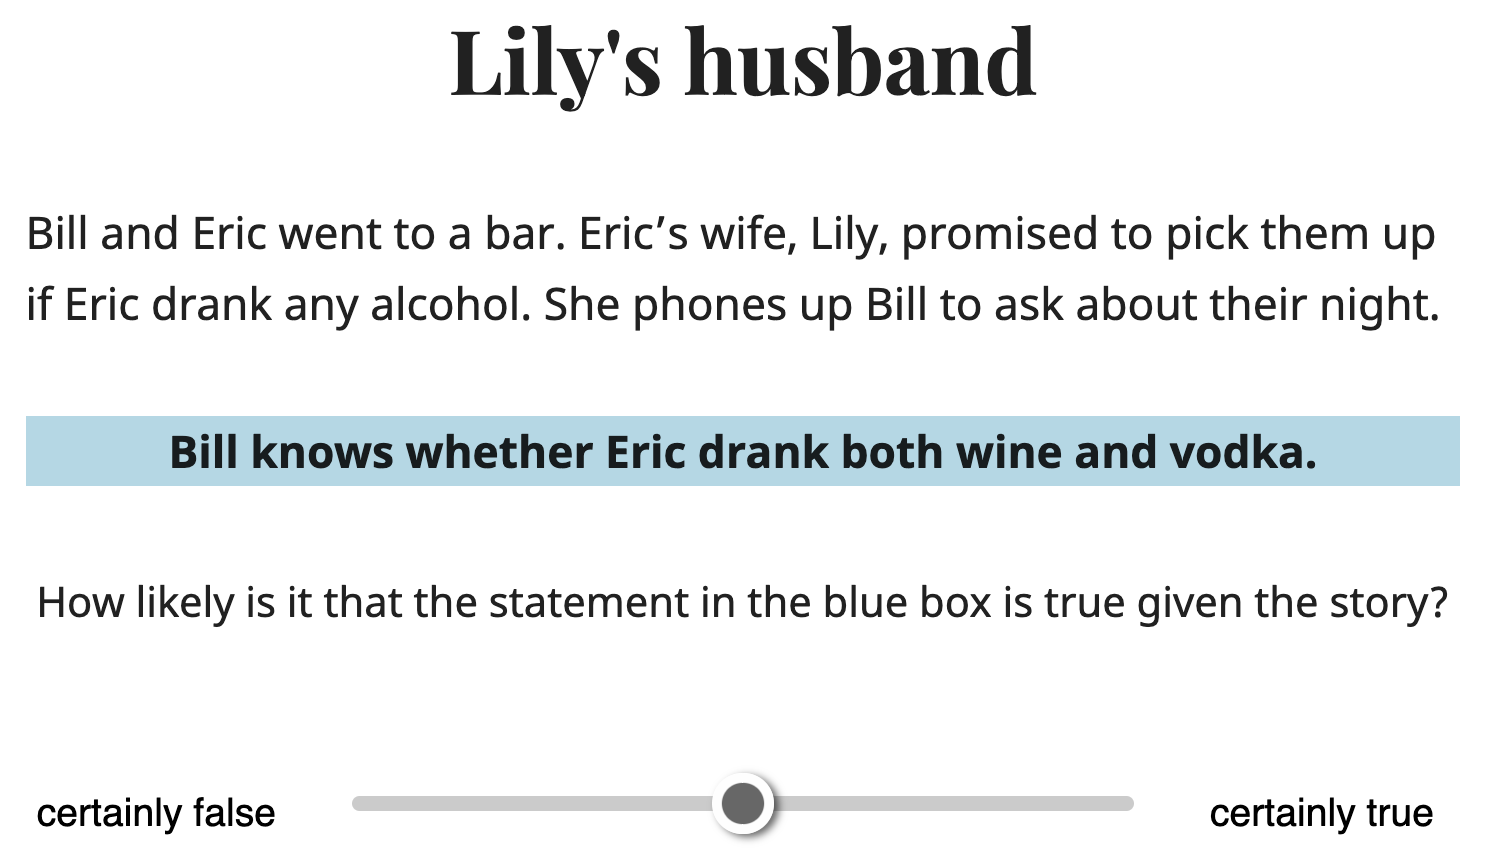
\includegraphics[width=0.8\linewidth]{images/screenshot_xor_comp.png}
 	\end{center}
 	\vspace{-0.3cm}
 	\caption{Example view of a trial eliciting the competence rating for an ``or''-vignette.}
 	\label{screenshot-xor-comp}
\end{figure}
\begin{figure}[h]
	\begin{center}
		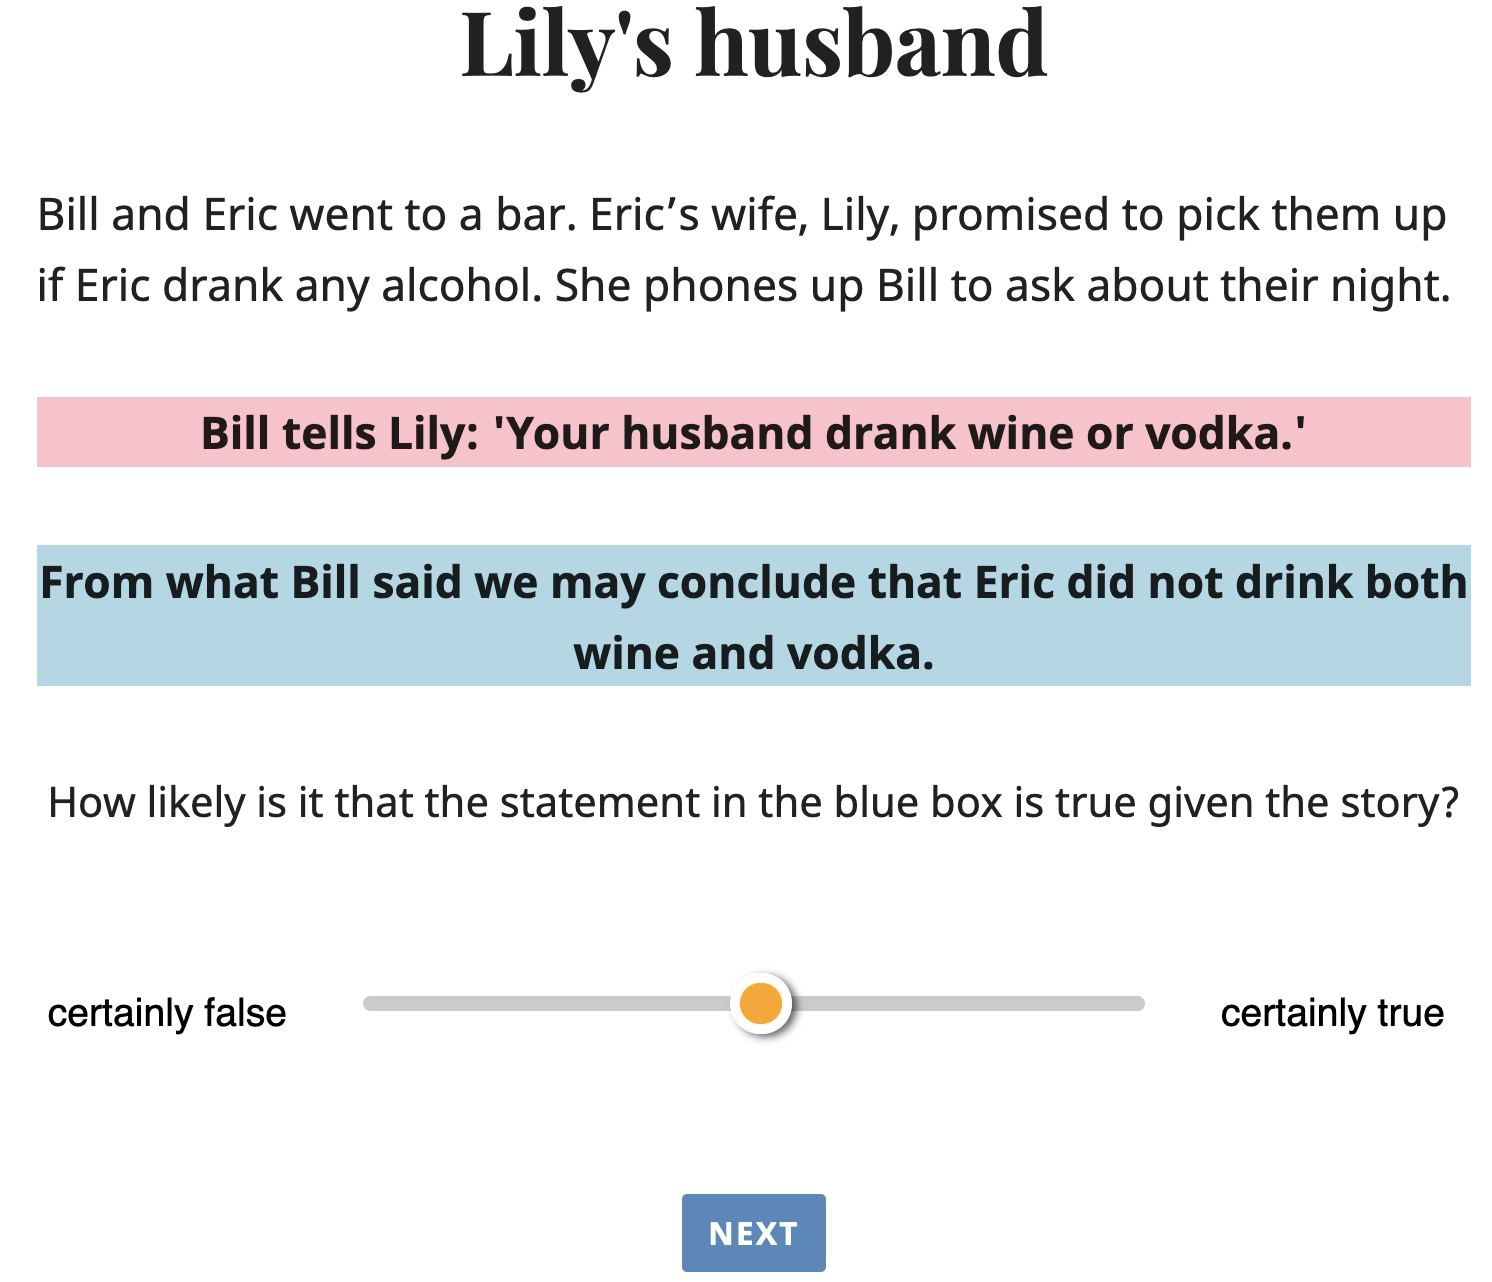
\includegraphics[width=0.8\linewidth]{images/screenshot_xor_target.png}
	\end{center}
	\vspace{-0.3cm}
	\caption{Example view of a trial eliciting the critical inference strength rating for an ``or''-vignette.}
	\label{screenshot-xor-target}
\end{figure}
 
Below, participants read the task saying ``How likely is it that the statement is true given the story?'', followed by a slider rating bar labelled ``certainly false'' (left) and ``certainly true'' (right). The continuous ratings were converted to an integer rating between 0 and 100 in the background. For each critical vignette, participants completed a block of 10 or 11 trials, consisting of a trial with a comprehension question, trials with statements eliciting relevance, comptenece and prior ratings each (the last factor was elicited with two statements for the trigger ``or''), followed by three more comprehension questions, and the critical implicature strength elicitation trial. 
Comprehension trials were visually identical to the critical trials, but the statement to be rated only referred to the content of the background stories, and were designed so as to be either clearly true, clearly false or uncertain given the background story. 
The four comprehension statements for one vignette were sampled at random from six possible statements (two per type true / false / uncertain). 
 
 We designed 32 different stories per trigger type (``some''~vs.~``or''), resulting in a total of 64 stories. Each subject saw eight randomly sampled stories (one per prior $\times$ competence $\times$ relevance condition out of four possible stories) such that they saw four ``or'' and four ``some'' stories in randomized order. The assignment of conditions to the triggers is randomized between-subjects.

At the beginning, participants were welcomed to the experiment, read instructions and first saw three labelled example trials showing the working of the slider. They read a simple story about a person shopping. They then saw a question about the story that was clearly false (expected rating: 0), clearly true (expected rating: 100) and implied to be rather true (expected rating: 50-100), given the background story. These expected responses were labelled and explained.  
The main part of the experiment consisted of eight critical stories, randomly shuffled with eight attention check stories. The attention checks consisted of one trial, visually matching critical trials. On these trials, the vignettes contained a statement which clearly wrote out what participants were supposed to answer (e.g., ``Please move the slider maximally left'') in an area of text that participants had to read to complete the trial. Participants who failed more than two of these attention checks were excluded from the analysis. 
%Each critical story block has the following structure: Participants read a background story, followed by a comprehension statement which is either clearly true, clearly false, or uncertain (sampled at random for each story) which they are asked to rate using the slider. Then, they read statements presented in a box colored blue associated with the factors of interest and rate it using a slider bar. The factors of interest are relevance, competence and prior, in randomized order within-participants. In the “or”-condition, the prior statement consists of two symmetrical conditional sentences (see example below). Then, participants answer another three comprehension questions. These are followed by the critical utterance containing “or” / “some” appearing in a box colored red. Below, the target statement gathering the likelihood of the exclusive disjunction / the upper-bounded reading of “some” (i.e., the likelihood of the implicature) appears. Again, they rate the target statement using the slider. The background story remains on the screen throughout the trials. 
After the study, participants could voluntarily fill out a socio-demographic questionnaire.
The experiment can be viewed under \texttt{https://magpie-xor-some.netlify.app/}. The preregistration for the experiment can be found under \texttt{https://osf.io/v7zjp}.

\subsection{Participants}
We recruited 277 participants through the crowd-sourcing platform Prolific. Participants were restricted to those whose first language included English, who previously took part in at least five other Prolific studies, and whose approval rate was at least 0.9, according to prescreening criteria of the platform. Participants took 20 minutes on average to complete the study and were compensated \pounds2.48 for their participation. Following our preregistered exclusion criteria, we excluded 15 participants for not indicating their native language, 3 participants for completing the study in under 8 minutes, 26 participants for failing more than 20\% of the attention checks, and 27 for failing more than 20\% of the comprehension questions. Due to a coding error of the comprehension questions, 206 participants were left post applying exclusion criteria, although the preregistered target sample size post exclusions was 200 subjects (see the power analysis section below for justification details).
%\mf{we should give some details about the power analysis or link to a document in the repository}
In the following analyses, data from the 206 participants is analysed.\footnote{All analyses were also conducted on data from 200 subject, excluding the last six submissions. No noteworthy quantitative or qualitative differences of the results were observed.}

\subsection{Sample size justification}
\mf{I suggest to move this paragraph to the appendix}
We conducted a power analysis in order to determine the minimal sample size required for a power of 0.8 of finding evidence for the conjunction of all factor hypotheses (relevance, competence and prior) predicted by the SI account, finding that at least 180 subjects were required. 

More specifically, we conducted a simulation-based Bayesian power analysis which aimed at determining how many participants are required in order to detect a theoretically motivated conjunctive effect of the predictors prior, relevance and competence with a confidence of at least 0.8. The simulations were based on an assumed effect size $\beta = 0.15$ for all predictors assuming $z$-scored data \citep[e.g.,][]{degen2015investigating}, and a Region Of Practical Equivalence (ROPE) $\delta = 0.05$ for judging evidence for the directionality of a coefficient given the data \citep{kruschke2014doing}. That is, we determined how many participants would be necessary such that for each factor $X$ the absolute value of the regression coefficients |$\beta_X$| for main factor $X$ would be larger than $\delta$.
The simulations were further based on the maximal desired model justified theoretically and by the design.\footnote{The maximal model in R syntax is: \texttt{rating = trigger * prior * competence * relevance}. The random effects were omitted for computational tractability reasons and due to the lack of well-founded estimates of group-level effect sizes.}

For this analysis, hypothetical experimental data representing the predictor effect rating was simulated by drawing four samples from a standard Normal distribution $\mathcal{N}(0,1)$ per simulated subject per trigger. Next, the target inference strength rating was modelled as a sample from a normal distribution with the mean computed as the sum of the simulated predictor values weighted by the assumed effect size (0.15). Then, the desired maximal Bayesian regression model was computed on the simulated data. The described steps were performed for a number of subjects ranging from 100 up to 340, increased iteratively in steps of 20. For each number of subjects, the model was re-computed on the simulated samples for $k=100$ iterations. For each iteration $i_k$, the conjunctive hypothesis of interest was tested. 
The power for the given number of participants was calculated as the proportion of iterations for which the conjunctive hypothesis was credible (i.e., if the posterior probability $P(\beta_X > \delta \mid D)$ was at least 0.95, for $\delta = 0.05$ was the parameter that defined our ROPE for the conjunction of all three predictor coefficients). The target proportion was 0.8.

We found that at least 180 subjects were required. To account for potential data collection artifacts, we aimed to recruit 200 participants passing our exclusion criteria.

\section{Results}
Prior to conducting statistical analyses, we preprocess the data by standardizing (or z-scoring) the responses within each factor (relevance, comptence, prior) for each participant. This is done to counterbalance possible by-participant responsiveness to particular factors, while keeping an anlysis advantageous to the scalar implicature account, since the standardization is applied across triggers. 

If our factor hypotheses are true, on average, we expect higher likelihood ratings for the statements eliciting relevance, competence and prior judgements given items in the respective high conditions. Critically, we expect higher likelihood ratings for the scalar implicature, if the relevance and comptenece in the item were judged as high and the prior of the alternative as low.

\mf{Give section overview: 4.1 plots and descriptive stats, 4.2 Confirmatory analyses following preregistration; 4.3 additional exploratory analyses (some of which preregistered?)}

\subsection{Predictor ratings}

\mf{I think that it would be great to have a plot, accompanying Figure~\ref{main-raw-ratings}, which shows ``idealized data according to assumed hypotheses''. So, how would the plot in the Figure look like if all of our predictions were borne out precisely? We could sample ``fictitious'' data and make a plot exactly like in Figure~\ref{posteriors-main}.}

\begin{figure}[h]
	\begin{center}
		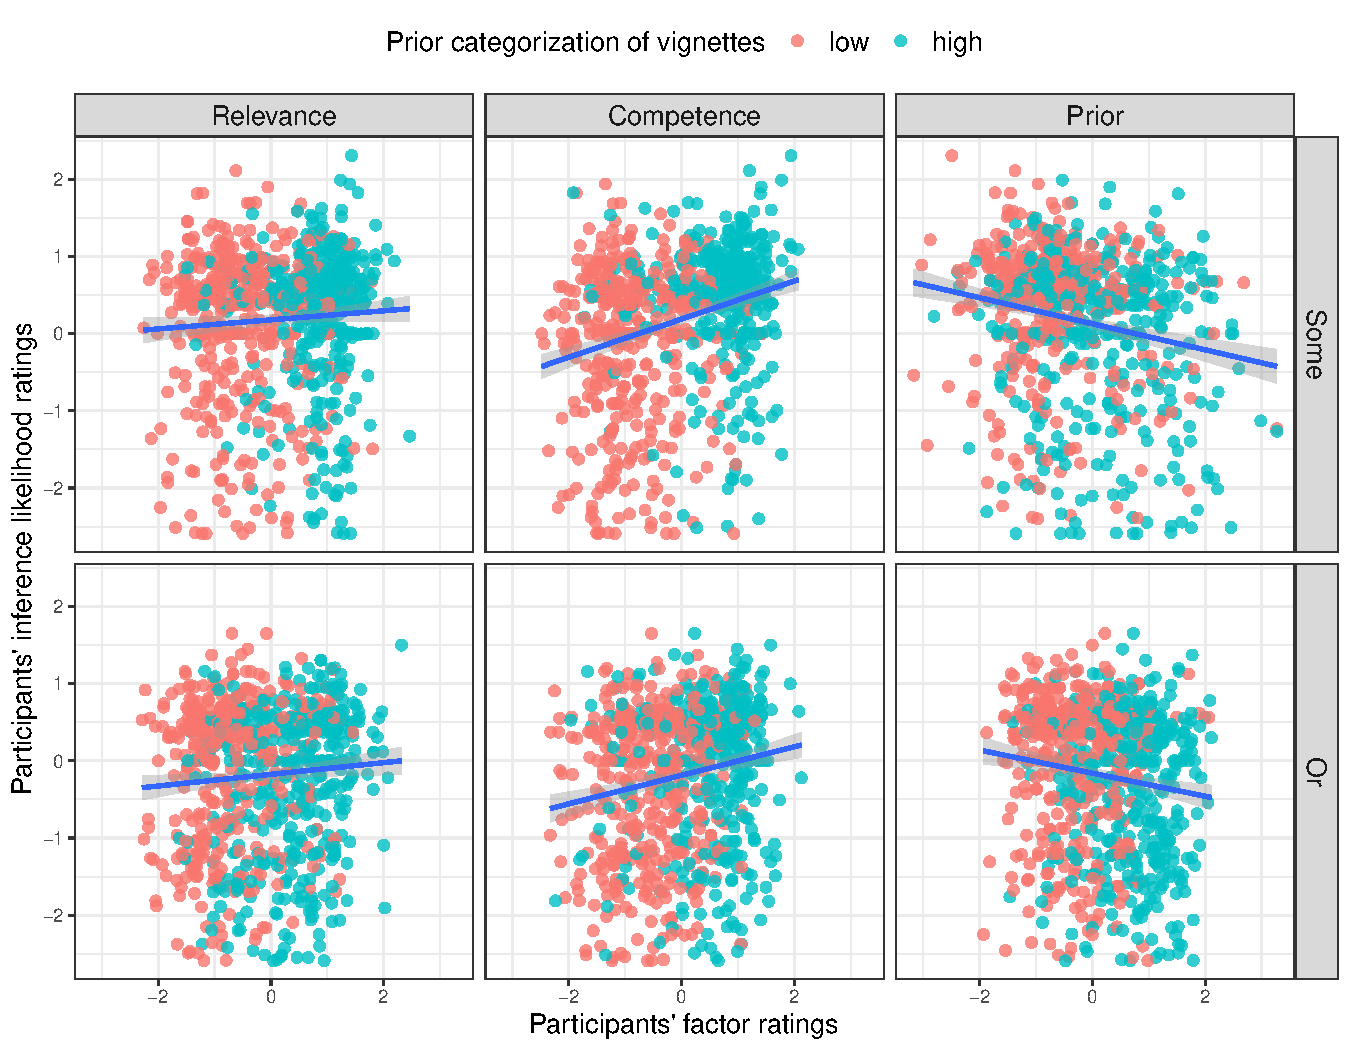
\includegraphics[width=1\linewidth]{images/byFactor-byPrior-raw-scatter.pdf}
	\end{center}
	\vspace{-0.3cm}
	\caption{Relating ratings for relevance, competence and prior statements (x-axis) to ratings for the strength of pragmatic enrichments (y-axis). The top row shows ratings for “some” (enriched to “some, but not all”). The bottom row shows ratings for “or” (enriched to “A or B, but not both”). Ratings for stories categorized as low (red) w.r.t. a given factor are on average lower (x-axis) than for those categorized as high (blue). The apparent effect of prior for “or” is mitigated by collinearity with relevance.}
	\label{main-raw-ratings}
\end{figure}


\begin{figure}[h]
	\begin{center}
		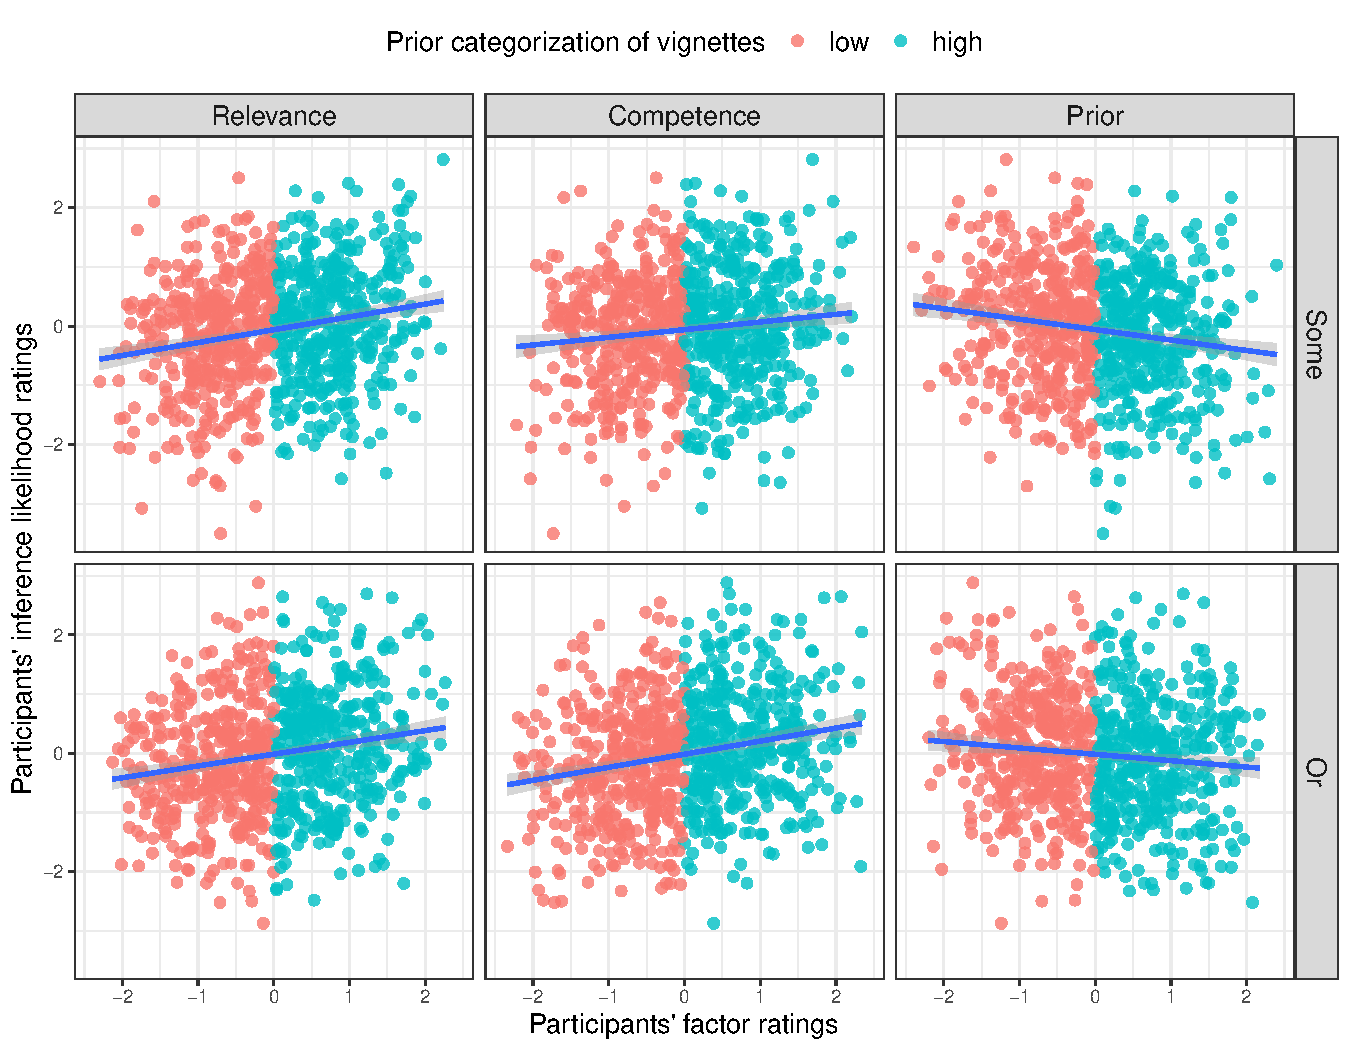
\includegraphics[width=1\linewidth]{images/idealized_data_N200_b015.pdf}
	\end{center}
	\vspace{-0.3cm}
	\caption{Simulated ratings for relevance, competence and prior statements (x-axis) in relation to ratings for the strength of pragmatic enrichments (y-axis). Ratings for stories categorized as low (red) w.r.t. a given factor are on average lower (x-axis) than for those categorized as high (blue).}
	\label{main-sim-ratings}
\end{figure}

Participants’ factor ratings by-story agreed well with the designed classification of the stories (Fig. \ref{main-raw-ratings}, red vs. blue color on $x$-axis). That is, the ratings for the relevance, comptence and prior statements were not distributed uniformly across the stories, but align with the prior categorization of the story for the respective factor (Fig. \ref{main-raw-ratings}). This provides validation for our experimental manipulation of the explanatory factors, as can be seen when comparing Fig. \ref{main-raw-ratings} with Fig. \ref{main-sim-ratings} which depicts idealized data (N=200) simulating perfectly borne out hypotheses. \pt{Like this?}

\subsection{Confirmatory analyses following preregistration}

We analysed the results using a Bayesian linear mixed effects model, regressing the target implicature rating against the fixed effects of predictor ratings (i.e., the relevance, comptence and prior ratings elicited by the same participant for that vignette), the effect of trigger and their two-, three-, and four-way interactions. Maximal computationally tractable random effects structure justified by the experimental design was included: we included random intercepts and random slope effects for the main effects of trigger, relevance, competence and prior by-subject, as well as random intercepts by-vignette.\footnote{Model in R syntax style: \texttt{inference-rating $\sim$ trigger * relevance * competence * prior + (1 + trigger + relevance + competence + prior || subjectID) + (1 | vignette)}. For computational tractability reasons, the correlation of random effects by-subject was set to 0.}
The categorical effect of trigger was dummy coded, using ``some'' as the reference level. For all regression coefficients we used a wide and uninformative prior given by a $t$-distribution with mean 0, standard deviation of 2 and 1 degree of freedom. The model was fitted using the R \texttt{brms} package \citep{burkner2017brms}.\footnote{The data and the analyses can be found under\newline \texttt{https://github.com/magpie-ea/magpie-xor-experiment}}

We focus on six slope coefficients of the regression model, for the effects of relevance, competence and prior, respectively, once for ``some'' and once for ``or''. We check whether the posterior estimate of each effect is in either one of three intervals: (1) negative effect ($\le$ -0.05), (2) no effect (between -0.05 and 0.05), or (3) positive effect ($\ge$ 0.05). We set the threshold for considering an effect as positive or negative to ±0.05 because we consider 0.05 to be the Region of Practical Equivalence (ROPE) for the effect sizes we expect \citep{kruschke2014doing}.
We interpret the data as providing evidence in favor of an effect (positive, negative, no effect) if the posterior probability of the effect being true is >= 0.95 (i.e., 95\% of posterior samples are in the corresponding interval). The probabilities of the respective coefficients lying in a particular interval are reported below (i.e., for instance, if $P=0.95$ is reported, it means that 95\% of the posterior samples of the given coefficient are in the respective interval). In particular, we speak of evidence in favor of the scalar implicature account of the exclusive disjunction interpretation if the posterior probability of the prior effect being negative, the relevance and competence effects being positive is $\ge$ 0.95. Example simulated posterior distributions over effect size samples which would confirm all our hypotheses can be seen in Fig. \ref{posteriors-sim}.

\begin{figure}[h]
	\begin{center}
		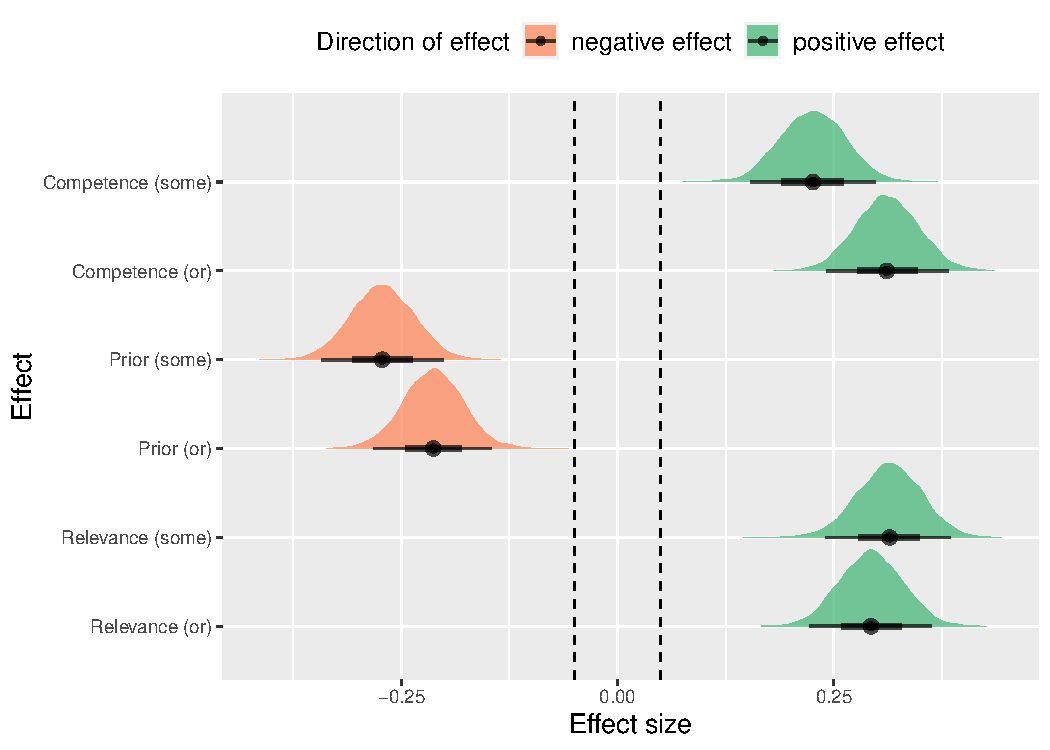
\includegraphics[width=1\linewidth]{images/posterior-effects-idealized-sim.pdf}
	\end{center}
	\vspace{-0.3cm}
	\caption{ \pt{How's this?} Simulated main analysis results which would confirm all hypotheses: Distributions of the posterior samples of each factor of interest for the trigger ``some'' and ``or''. The effect size was set to 0.25 and matches Fig. \ref{main-sim-ratings} for visualization purposes. The colors and the vertical dashed lines indicate the effect intervalls (from left to right: negative, no, positive effect). Points indicate posterior means, thick lines indicate 66\% credible intervals, thin lines indicate 95\% credible intervals.}
	\label{posteriors-sim}
\end{figure}


\begin{figure}[h]
	\begin{center}
		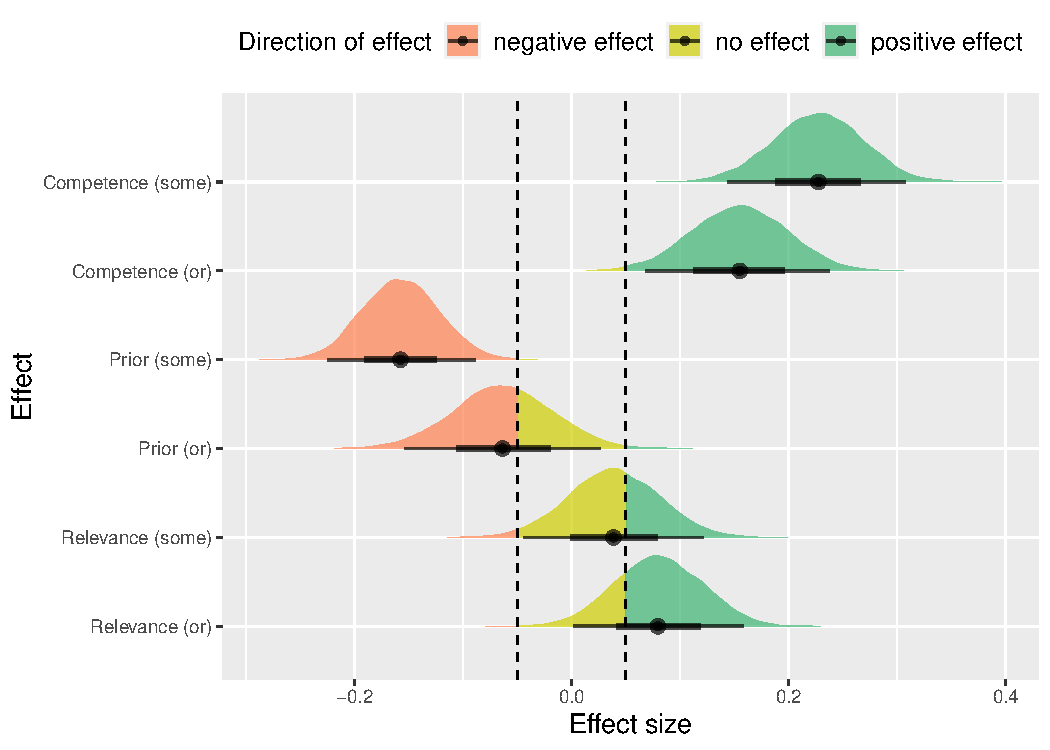
\includegraphics[width=1\linewidth]{images/posterior-effects-noDupl.pdf}
	\end{center}
	\vspace{-0.3cm}
	\caption{Main analysis results: Distributions of the posterior samples of each factor of interest for the trigger ``some'' and ``or''. The colors and the vertical dashed lines indicate the effect intervalls (from left to right: negative, no, positive effect). Points indicate posterior means, thick lines indicate 66\% credible intervals, thin lines indicate 95\% credible intervals.}
	\label{posteriors-main}
\end{figure}

\begin{table}
  \centering
   \begin{tabular}{llccc}
           &            & negative & no effect & positive \\ \midrule
    {some} & relevance  & 0.019    & 0.592       & 0.389      \\
           & competence & 0        & 0         & 1        \\
           & prior      & 0.999        & 0.001     & 0    \\
    {or}   & relevance  & 0     & 0.228       & 0.772      \\
           & competence & 0      & 0.007       & 0.993      \\
           & prior      & 0.619    & 0.373       & 0.008      \\
   \end{tabular}
  \caption{Results of confirmatory analysis.}
  \label{tab:results-confirmatory}
\end{table}

Results from this analysis are summarized in Table \ref{tab:results-confirmatory}.
Consistent with predictions, for the trigger ``some'', we find a clear negative prior probabilty effect of the stronger alternative ``all'' being true, as inidcated by the probability of the negative effect of prior being $P = 0.999$ (Fig.\ref{posteriors-main}, \texttt{Prior~(some)} line, orange color). Similarly, we find a clear positive effect for speaker competence ($P =  1$, Fig.\ref{posteriors-main}, \texttt{Competence~(some)} line, green color). However, we do not find any clear effects of relevance (Fig.\ref{posteriors-main}, \texttt{Relevance~(some)} line, split colors). If anything, the data supports the hypothesis that the effect is not negative.


For the trigger ``or'', in contrast, we only find a positive effect of competence ($P =  0.993$, Fig.\ref{posteriors-main}, \texttt{Competence~(or)} line, green color).  We find no comprehensive effects for relevance or competence. While the reason for the former might be the same as for ``some'', we suggest that these results might also be influenced by collinearity of the effects. We turn to this conjecture in light of the exploratory analyses, described below. 
Overall, these results would provide evidence against the scalar implicature hypothesis because not all factors yielded an effect on the robustness of scalar implicatures generated from ``some'' and ``or''. Similarly, the results would provide evidence against the identity hypothesis, as an effect of prior was observed for ``some'', but not for ``or''.

\subsection{Exploratory analyses}

\subsubsection{Models with alternative predictors}

\begin{figure}[h]
	\begin{center}
		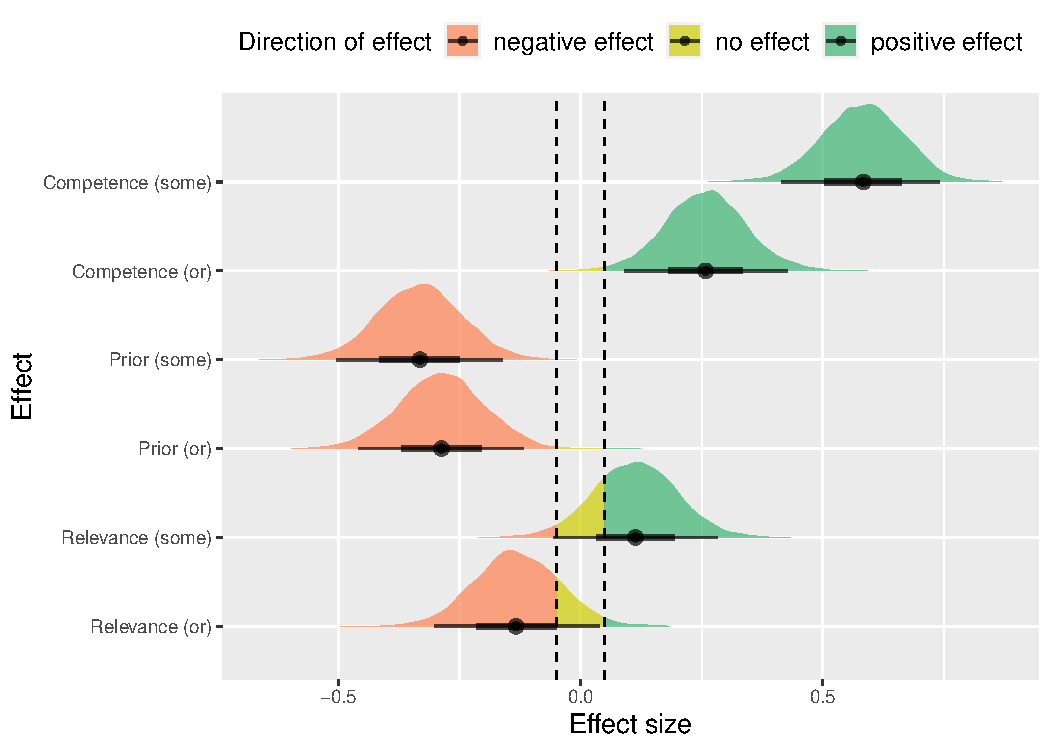
\includegraphics[width=1\linewidth]{images/posterior-effects-categorical-noDupl.pdf}
	\end{center}
	\vspace{-0.3cm}
	\caption{Exploratory analysis with categorical predictors: Distributions of the posterior samples of each factor of interest for the trigger ``some'' and ``or''. The colors and the vertical dashed lines indicate the effect intervalls (from left to right: negative, no, positive effect). Points indicate posterior means, thick lines indicate 66\% credible intervals, thin lines indicate 95\% credible intervals. \mf{I'm not sure if we should blindly reuse a threshold of 0.05 here without further justification. Something to think about.}}
	\label{posteriors-cat}
\end{figure}

In order to further investigate the relevance effects and potential collinarity concerns, we computed exploratory pairwise correlations of all the predictors. Interestingly, we find a significant correlation between the prior and the relevance effects for the trigger ``or'' ($R^2 = -0.106$). We also found a significant correlation between competence and relevance ($R^2 = 0.127$) for ``or''. \pt{We should talk about the latter correlation in more detail at some point.} No correlations were found for ``some''. These intriguing results might indicate that these effects are closely related for disjunction. Intuitively, a negative correlation between prior and relevance of the stronger alternative ``and'' makes sense: the more likely the conjunction is a priori, the more likely it is that the listener might know about it already, yielding the implicature irrelevant to the listener. Similarly, competence might be connected to relevance indirectly via the prior: the more likely the stronger alternative is a priori, the more likely it is that a speaker knows about it, while the irrelevance still persists for the listener. However, these speculations call for further research. \mf{I suggest removing the last sentence here and to pick this up in the general discussion, together with Bob's worry that we lack an explanation for why there is no such correlation in the case of ``some''.}

In addition to the main analysis, we conducted three exploratory regression analyses, which shed more light on the concerns of collinearity. First, we fit a model using categorical predictors only. That is, we fit a Bayesian linear mixed effects regression model, regressing the inference rating against our prior intuitive classifications of the vignettes on the dimensions relevance, competence and prior (high or low, respectively), the effect of trigger, and their interactions. The random effects structure and the priors were identical to the main model. The factors were sum-coded, -1 representing the low condition, 1 representing the high condition.
This model decouples the predictors by dichotomizing their classification and, therefore, addresses the potential collinearty issue. Furthermore, it provides a comparison between participants' judgements and our intuitive prior classifications of the vignettes. 

Given this model and the data, we found very similar results for both triggers: We observe a negative effect of prior and a positive effect of competence, in line with predictions of the scalar implicature hypothesis (Fig.~\ref{posteriors-cat}). However, we again observe no effects of relevance. If anything, the relevance effect tends in the direction opposite to predictions of the SI account for the trigger ``or''. 

\begin{figure}[h]
	\begin{center}
		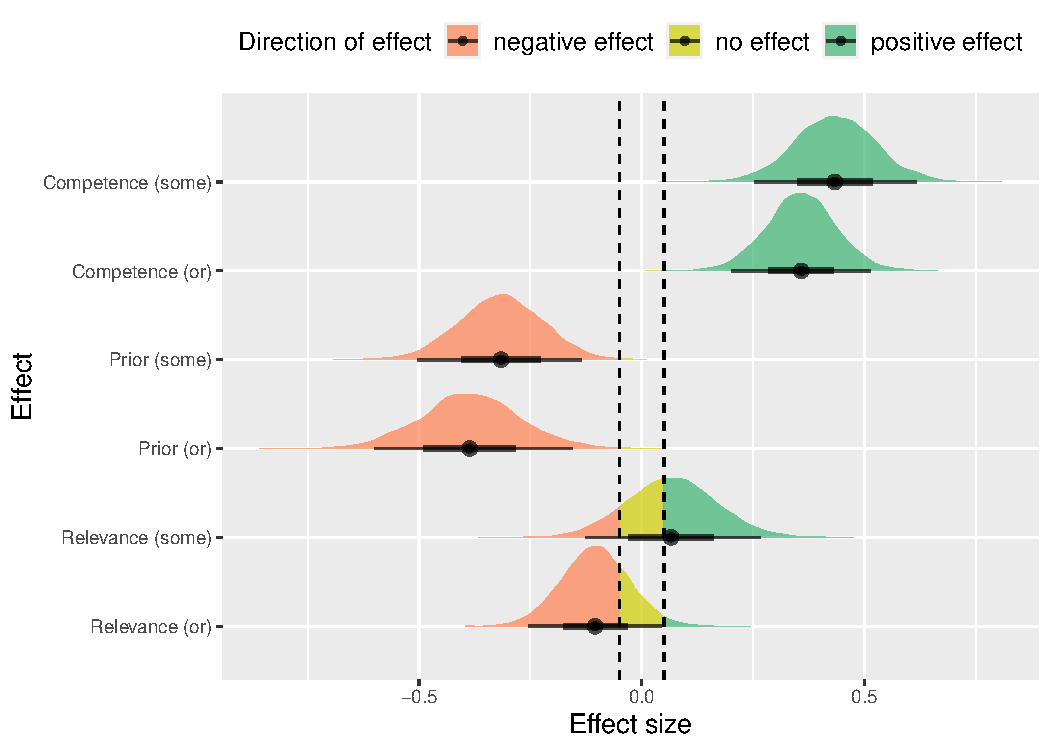
\includegraphics[width=1\linewidth]{images/posterior-effects-means-noDupl.pdf}
	\end{center}
	\vspace{-0.3cm}
	\caption{Exploratory analysis with predictor ratings averaged by-vignette: Distributions of the posterior samples of each factor of interest for the trigger ``some'' and ``or''. The colors and the vertical dashed lines indicate the effect intervalls (from left to right: negative, no, positive effect). Points indicate posterior means, thick lines indicate 66\% credible intervals, thin lines indicate 95\% credible intervals. \mf{I'm not sure if we should blindly reuse a threshold of 0.05 here without further justification. Something to think about.}}
	\label{posteriors-mean}
\end{figure}

These results match the second exploratory analysis, whereby the ratings were used as predictors in the linear model, but the ratings were averaged for each vignette across participants. In this second  exploratory model, we again find similar effects for ``some'' and ``or'': a positive effect of competence, negative for prior, and an indefinite relevance effect (Fig.~\ref{posteriors-mean}). By averaging over single participant ratings, this model indicates that the absent competence effect for the disjunction in the main model might be due to by-participant variation.


Finally, we conduct an exploratory analysis when setting the ROPE to 0. That is, we investigate whether the posterior estimates for the regression coefficients of interest are positive ($>0$) or negative ($<0$) and interpret the data as providing evidence in favor of a particular direction if at least 95\% of posterior samples for the respective coefficent are positive or negative. As in the main analysis, we find credible positive effects of competence for both ``some'' ($P = 1$) and ``or'' ($P = 1$), and a credible negative effect of prior for ``some'' ($P = 1$), but not for ``or'' ($P=0.91$). However, in contrast to the main analysis, we do find a credible positive effect of relevance for ``or'' ($P=0.978$), but not for ``some'' ($P=0.829$). \pt{We should include justification for using a ROPE in the first place here. Some more discussion needs to be added too.} 

\pt{We have a generally higher rate of implicature generations for ``some'' than for ``or'' (across conditions): the average inference likelihood rating for the former is 0.179, and -0.179 for the latter. Maybe something to mention in the discussion}

\subsubsection{Model comparisons}
Because the correlations hint at possible collinearity effects between relevance and prior for the trigger ``or'', we conduct exploratory model comparisons. That is, in order to check whether certain factors among relevance, competence and prior have a stronger influence on the inference stength ratings than others, we compare regression models of different complexity. We take a Bayesian approach to model comparison here in terms of their Bayes factors \citep{rouder2012default}.
We compare all regression models that can be built with the three explanatory factors as main factors against a baseline intercept-only model.\footnote{If the model contains more than one main effect, all interactions between main effects are always included in the model, as well. All justified and computationally tractable random effects are added to each model, respectively.}
Following literature, we interpret the evidence in favor of a particular model as strong if the odds (i.e., the Bayes Factor) are above 10 or below 1/10; as mild, if they are between 3 and 10 or 1/3 and 1/10; and as absent if the odds are between 3 and 1/3 \citep[e.g.,][]{lodewyckx2011tutorial}. 

\begin{figure}[h]
	\begin{center}
		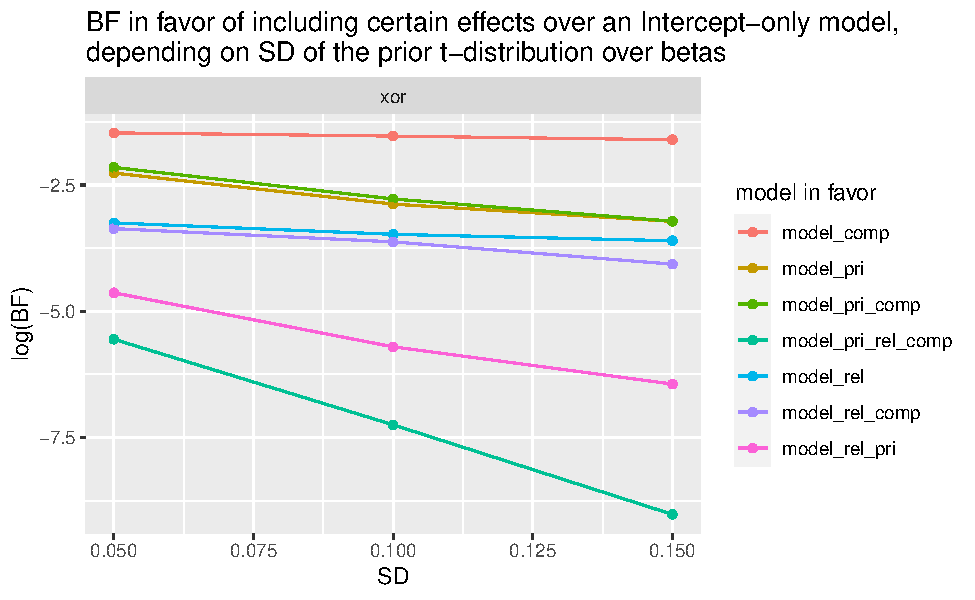
\includegraphics[width=\linewidth]{images/BF_vs_SD_allModels_vs_int.pdf}
	\end{center}
	\vspace{-0.3cm}
	\caption{Bayes factor comparison of different main factor combinations (colors) for different standard deviation parameter values of the prior $t-$distribution over the main regression coefficients (x-axis). The log Bayes Factor (y-axis) is computed in favor the more complex model over an intercept-only model. \pt{Model names will be made human-readable, the title will be removed.}}
	\label{bf-grid-search}
\end{figure}

To investigate the stability of the Bayes factors of a certain model over the baseline, we conduct a grid search over the standard deviation parameter of the prior $t$-distribution over the main effect regression coefficients. More precisely, given that the expected effect size for the main factors was around $\beta=0.15$, the standard deviation parameters considered in the grid search included {0.05, 0.1, 0.15}. Figure \ref{bf-grid-search} shows the Bayes factors against the intercept-only model of all the regression models plotted against the different standard deviation parameters of the priors. It indicates that, in general, the Bayes factor does not change strongly dependent on the tightness of the prior distribution. It further suggests that the intercept-only model is a better fit to the data than all of the explored regression models, but more so for models containing both relevance and prior as explanatory factors. This corroborates the finding based on the correlation, indicating that relevance and prior might be co-dependent and explain each other away. We also observe that models containing the effect of relevance are slightly less likely given the data than models containing the effect of prior, but the difference is negligible. However, these results might also be due to the fact that additional model complexity of the regression models overpowers potential improvement in model fit.

\begin{figure}[h]
	\begin{center}
		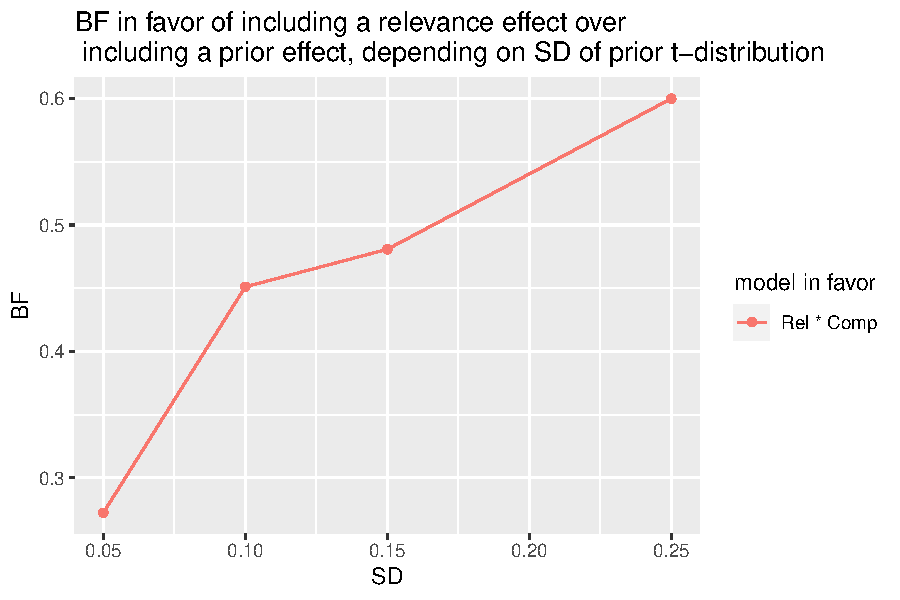
\includegraphics[width=\linewidth]{images/BF_vs_SD_rel-comp_pri-comp.pdf}
	\end{center}
	\vspace{-0.3cm}
	\caption{Bayes factor of the \texttt{relevance*competence} model over the \texttt{prior*competence model} (y-axis), plotted against different standard deviation parameter values of the prior $t-$distribution over the main regression coefficients (x-axis). \pt{The title will be removed.}}
	\label{bf-rel-pri}
\end{figure}

Therefore, to zoom in on the comparison between the effects of relevance and prior on inference strength ratings we conduct further exploratory model comparisons. Specifically, we compare two-factor models, comparing relevance over prior, each combined with competence, respectively. As can be seen in Figure \ref{bf-rel-pri}, the Bayes factor varies more strongly depending on the standard deviation parameter of the prior distribution over the main regression coefficients. For $SD=0.05$, we find $BF=0.27$, indicating that the model containing  the predictors \texttt{prior*competence } is made around three times more likely than the \texttt{relevance*competence} model, which can we consider mild evidence in favor of prior being the better predictor for the inference strength of exclusive disjunctions.
Yet further investigation of the interaction between relavance and competence effects with respect to their influence on exclusive disjunctions is needed.
 
\section{Discussion}
In sum, the results provide moderate evidence for the scalar implicature account of ``some'' and ``or''. While we could confirm the effects of prior and comptence for the interpretation of ``some'' as predicted by the SI hypothesis, we could not verify them for the disjunction. We also did not find evidence for effects of relevance on the robustness of scalar implicature generation, given the vignettes. We hypothesize that the absense of a clear-cut relevance effect might be due to the difficulty manipulating this dimension contextually. It might be that the vignettes used in the experiment failed to make the listener relevance salient enough for any effects to be borne out. Further experiments should improve this manipulation, as well as additionally consider speaker relevance.

Furthermore, our results hint at intriguing dependencies between relevance and prior effects for the interpretation of exclusive disjunctions. Taken together, the results might speak against the identity hypothesis, indicating that there might be subtle differences in the conceptualization of the stronger alternative for ``some'' and ``or''. \pt{Focus on the aspect of interactions between the predictors more strongly.}

\section{Appendix}
\subsection{Vignettes}
\pt{Include all the vignettes?}

\bibliography{paper.bib}

\begin{addresses}
  \begin{address}
    Author1 Full Name \\
    Street \\
    City, State Zip \ldots \\
    \email{author1@example.org}
  \end{address}
  % Repeat or remove additional addresses as needed.
  \begin{address}
    Author2 Full Name \\
    Street \\
    City, State Zip \dots \\
    \email{author2@example.com}
  \end{address}
\end{addresses}

\end{document}
